\documentclass[a4paper,11pt]{paper}

\usepackage[pdftex]{graphicx}
\usepackage{color}

\title{ColouredTree: a BEAST 2 framework for describing
phylogenies within structured populations}

\author{Tim Vaughan}

\newcommand{\class}[1]{\textsf{#1}}
\newcommand{\project}[1]{\textsf{#1}}
\newcommand{\inp}[1]{\textsf{\color{blue}#1}}
\newcommand{\code}[1]{\texttt{#1}}

\begin{document}

\maketitle

\section{Introduction}

BEAST 2 (hereafter simply referred to as BEAST) currently provides no
native way of handling true coloured trees---i.e., phylogenetic trees
corresponding to lineages evolving within some kind of structured
population. While it is true that BEAST has a useful facility for
recording arbitrary metadata in the form of ``traits'' on tree nodes,
information cannot be modified by BEAST Operators.  Without this
capability, geographic model parameters such as migration rates are
beyond the scope of the inference apparatus.

This document describes some first steps towards addressing these
shortcommings.

\section{State of the project}
Before going into the details of the plugin itself, let's consider the
current state of the development. So far, we have in place
\begin{itemize}
	\item a plugin for representing coloured trees,
	\item a plugin for initialising coloured trees from the structured
		coalescent, and
	\item a means of visualising coloured trees using Alexei's
		\project{beast-graphics} project.
\end{itemize}
These are the items which are described in the present document.

On the to-do list are the following (more challenging) items:
\begin{itemize}
	\item proposal operators for modifying colour assignments,
	\item calculation nodes for determining likelihoods of particular
		colour assignments.
\end{itemize}
Note that specific likelihoods and proposal operators depend on the
underlying structural model the colours represent, so we firstly need
to implement a general framework for such operators, then implement
some specific common cases (such as those relating to models of
migration between demes).

\section{Implementation of Coloured Trees (ColouredTree plugin)}

\begin{figure}
	\centering
	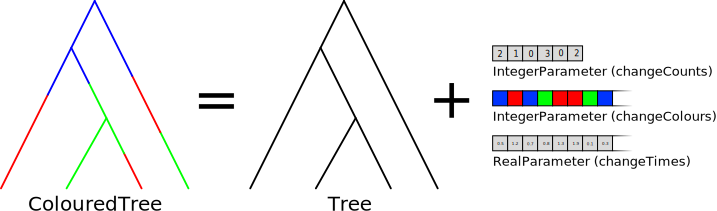
\includegraphics[width=\textwidth]{treeComposition.pdf}
	\caption{Composition of the \class{ColouredTree} plugin.}
	\label{fig:ColouredTree}
\end{figure}

The first and most important point about the way in which coloured
trees are implemented is that the main class, \class{ColouredTree},
extends \class{Plugin}---it does not extend \class{Tree}.  As such,
\class{ColouredTree}s are not \class{StateNodes}, and cannot be used
directly in an MCMC calculation.  Instead, \class{ColouredTree} takes
a \class{Tree} as the input \inp{tree}, along with three parameter
arrays which are used to record the colouring information. (This
structure is illustrated in Fig.~\ref{fig:ColouredTree}.) The three
parameter array inputs are:
\begin{description}
	\item[\inp{changeCounts}]: an \class{IntegerParameter} array which
		is used to record the number of colour changes along each
		branch,
	\item[\inp{changeColours}]: another \class{IntegerParameter}
		array used to record the actual colours each change results
		in, and
	\item[\inp{changeTimes}]: a \class{RealParameter} array used to
		record the times (heights) at which the colour change events
		occur. \emph{Note: absolute times rather than time differences
		are recorded}.
\end{description}

The counts in the \inp{changeCounts} array are indexed by the node
numbers (obtained via \code{node.getNodeNr()}) of the nodes on the
leaf-side of each branch.  The length of this array is equal to the
number of branches in \inp{tree}.

The colours in \inp{changeColours} and times in \inp{changeTimes} are
stored as flattened matrices, with the row identified by the leaf-side
node number and the column given by a number between 0 and one less
than the change count for the branch specifying that particular
change. Note that as the total length of \class{Parameter} arrays
cannot change once they are initialised, the dimension of
\inp{changeTimes} and \inp{changeColours} must be fixed.  It is thus
necessary to set an upper bound on the total number of changes which
can occur along any branch, and this is specified via the input
\inp{maxBranchColours}.

Clearly the way in which the colour information is stored in these
\class{Parameters} fairly cumbersome. This is a necessary evil
as, unlike \class{ColouredTree}, \class{Parameter}s \emph{do} extend
\class{StateNode} and may thus form part of the state in an MCMC
calculation. However, they should not be accessed directly either by
\class{Operator}s or methods involved in the creation of
\class{ColouredTree} objects. Instead, \class{ColouredTree} exposes a
set of helper methods which allow the colouring information to be
handled in a more intuitive way.

\subsection{Other ColouredTree inputs}

Before moving on to describing these helper methods, however, we will
briefly describe the other inputs to \class{ColouredTree}.

\begin{description}

	\item[\inp{colourLabel}]: a \class{String} for providing a
		single word description of what different colours mean. (E.g.
		``deme''.) This is used to label the colour metadata in trees
		generated by \code{getFlattenedTree()}, as described below.

	\item[\inp{nColours}]: an \class{Integer} input used to fix the
		total number of distinct colours.

	\item[\inp{leafColours}]: an \class{IntegerParameter} array
		containing the fixed colours at each of the leaves of
		\inp{tree}.

\end{description}

\subsection{ColouredTree helper methods}

Besides the usual \code{initAndValidate()}, \class{ColouredTree}
provides a number of methods for accessing and modifying the colouring
of a tree. The most important of these methods are:

\begin{description}
	\item[\code{getLeafColour(Node node)}]: Returns the colour
		associated with a leaf node.

	\item[\code{setChangeCount(Node node, int newCount)}]: Sets the
			number of changes along the branch between node and its
			parent.

	\item[\code{setChangeColour(Node node, int change, int
		newColour)}]: Sets colour of change number \code{change} on the branch
		between \code{node} and its parent to \code{newColour}.
	

	\item[\code{setChangeTime(Node node, int change, double newTime)}]:
		Sets time of change number \code{change} on the
		branch between \code{node} and its parent to \code{newTime}.
	
	\item[\code{getChange*}]: Retrieve rather than set the counts,
		colours and times.

	\item[\code{addChange(Node node, int newColour, double time)}]:
		Adds a new colour change to the branch between \code{node} and
		its parent to colour \code{newColour} and at time \code{time}.

	\item[\code{getFlattenedTree()}]: This method creates a new
		\class{Tree} object in which the colour changes are recorded
		as single-child nodes in the tree. The colours along each
		sub-branch (between nodes in the new tree) are stored as
		meta-data affixed to the node at the leaf-side end of the
		branch, with the trait label specified by \inp{colourLabel}.

	\item[\code{valid()}]: Checks the internal consistency of the tree
		colouring (both times and colour changes) and returns True if
		a problem is found, False otherwise.

\end{description}


\section{Generating Coloured Trees (StructuredCoalescentColouredTree plugin)}

The \class{StructuredCoalescentColouredTree} plugin generates
\class{ColouredTree}s according consistent with the structured
coalescent.  It is a reimplementation of the
\class{StructuredCoalescentTree} plugin which generates regular BEAST
\class{Tree}s with colouring information stored in \class{Node}
metadata. It exists for two reasons:
\begin{enumerate}
	\item to provide a means of initialising \class{ColouredTree}s
		with colours consistent with a known set of leaf colours and with the
		particular structure of a migration rate matrix, and
	\item to provide a first test of the new \class{ColouredTree}
		plugin and its associated helper methods.
\end{enumerate}

Note that \class{StructuredCoalescentColouredTree} actually extends
\class{ColouredTree} so that it may be used to fill any input where a
coloured tree is required.

\subsection{StructuredCoalescentColouredTree inputs}

As \class{StructuredCoalescentColouredTree} is a reimplementation of
\class{StructuredCoalescentTree}, the inputs are essentially the same:

\begin{description}
	\item[\inp{rateMatrix}]: \class{RealParameter} matrix containing
		migration rates between distinct colours/demes.  Values along
		the diagonal are ignored.
	\item[\inp{popSizes}]: \class{RealParameter} array containing the
		fixed sizes of each of the differently coloured populations.
\end{description}

\subsection{StructuredCoalescentColouredTree methods}

This plugin doesn't have any additional methods which are interesting
from a user's perspective beyond those which it inherits from
\class{ColouredTree}.  The simulation is run by the
\code{initAndValidate()} method and used to populate the
\class{ColouredTree} inputs.

Note that due to the fact that, strictly speaking (in a Dutch accent),
only \class{Operators} are allowed to modify \class{StateNode} values,
\code{initAndValidate()} creates a local instance of \class{State} and
assigns the \class{ColouredTree} colour \class{Parameters} to it
before calling the \code{simulateTree()} method which actually
performs the structured coalescent calculation.  Remco is a little
worried that this may cause problems down the track when bona fide
\class{State}s are also floating around, so this is something we may
have to pay close attention to.

\section{Interfacing with {\textsf beast-graphics} (FlatColouredTree plugin)}

\begin{figure}
	\centering
	\includegraphics[width=0.5\textwidth]{structuredCoalescentFig.pdf}
	\caption{Coloured tree generated using
		\class{StructuredCoalescentColouredTree} and visualised using
	\project{beast-graphics} via the \class{FlatColouredTree} plugin.}
	\label{fig:structuredCoalescent}
\end{figure}

In order to visualise instances of \class{ColouredTree} initialised
using \class{StructuredCoalescentColouredTree} or via some other
means, we can use Alexei's awesome \project{beast-graphics} package.
However, this package only works with regular BEAST \class{Tree}s
with colouring information stored as meta-data on single-child nodes,
as described previously.

The \class{FlatColouredTree} plugin, which extends \class{Tree}, acts
as a stand-in for \class{ColouredTree}s to allow the colouring
information they contain to be passed to \class{Plugin}s which expect
this older style of coloured tree.

\subsection{FlatColouredTree inputs}

The \class{FlatColouredTree} only has a single input, \inp{treeColour}

\subsection{FlatColouredTree methods}

\end{document}
